Nella fase 3 hanno luogo i seguenti incrementi:
\begin{itemize}
	\item Incremento 1
	\begin{itemize}
		\item normazione: modifiche alle \textit{NormeDiProgetto\_v2.0.0} secondo quanto segnalato alla Revisione di Progettazione. Si procede poi con il suo incremento;
		\item pianificazione della qualifica: modifiche al \textit{PianoDiQualifica\_v2.0.0} secondo quanto segnalato alla Revisione di Progettazione. Si procede poi con il suo incremento;
		\item pianificazione delle attività: modifiche al \textit{PianoDiProgetto\_v2.0.0} secondo quanto segnalato alla Revisione di Progettazione;
	\end{itemize}
	\item Incremento 2, Incremento 3 e Incremento 4
	\begin{itemize}
		\item progettazione di dettaglio: incremento alla \textit{Technology Baseline} con i requisiti indicati nella tabella 3;
		\item codifica: codifica degli incrementi effettuati durante la progettazione;
		\item redazione manuali: incrementi al \textit{ManualeUtente\_v0.1.0} e al \textit{ManualeSviluppatore\_v0.1.0} in base a quanto segnalato alla Revisione di Qualifica;
		\item verifica: verifica degli incrementi effettuati;
	\end{itemize}
	\item Incremento 5
	\begin{itemize}
		\item Documentazione;
		\item Verifica documentazione;
	\end{itemize}
	\item validazione e collaudo: vengono eseguiti i test di qualifica e il collaudo per il rilascio;
	\item preparazione alla presentazione;
	\item approvazione dei documenti da parte del responsabile. Sono pronti per il rilascio le \textit{NormeDiProgetto\_v3.0.0}, il \textit{PianoDiProgetto\_v3.0.0}, il \textit{PianoDiQualifica\_v3.0.0}, l'\textit{AnalisiDeiRequisiti\_v3.0.0} il
	\textit{ManualeUtente\_v0.1.0} e il \textit{ManualeSviluppatore\_v0.1.0};
\end{itemize}

\begin{tabularx}{\textwidth}{| c | c | c | }
		\rowcolor{LightBlue}
		\color{white}\bfseries Incremento 2 & 
		\color{white}\bfseries Incremento 3 & 
		\color{white}\bfseries Incremento 4 \\[0.25cm]
		ROF1 & ROF7 & ROF22 \\ 
		ROF2 & ROF8 & ROF27 \\ 
		ROF3 & ROF9 & ROF28 \\ 
		ROF4 & ROF10 & ROF29 \\ 
		ROF5 & ROF11 & RDF1 \\ 
		ROF6 & ROF12 & RDF2\\ 
		ROF23 & ROF13 & RDF3 \\ 
		ROF24 & ROF14 &  RDF4\\ 
		ROF25 & ROF15 &  RDF7\\ 
		ROF26 & ROF16 &  RDF8\\ 
		ROF33 & ROF17 & RDF9 \\ 
		& ROF18 & RPF15 \\ 
		& ROF19 & RPF16\\ 
		& ROF20 & \\ 
		& ROF21 & \\  \hline
		\caption{Requisiti da soddisfare in fase 3}
	\end{tabularx}
	

\begin{figure}[h]
	\centering
	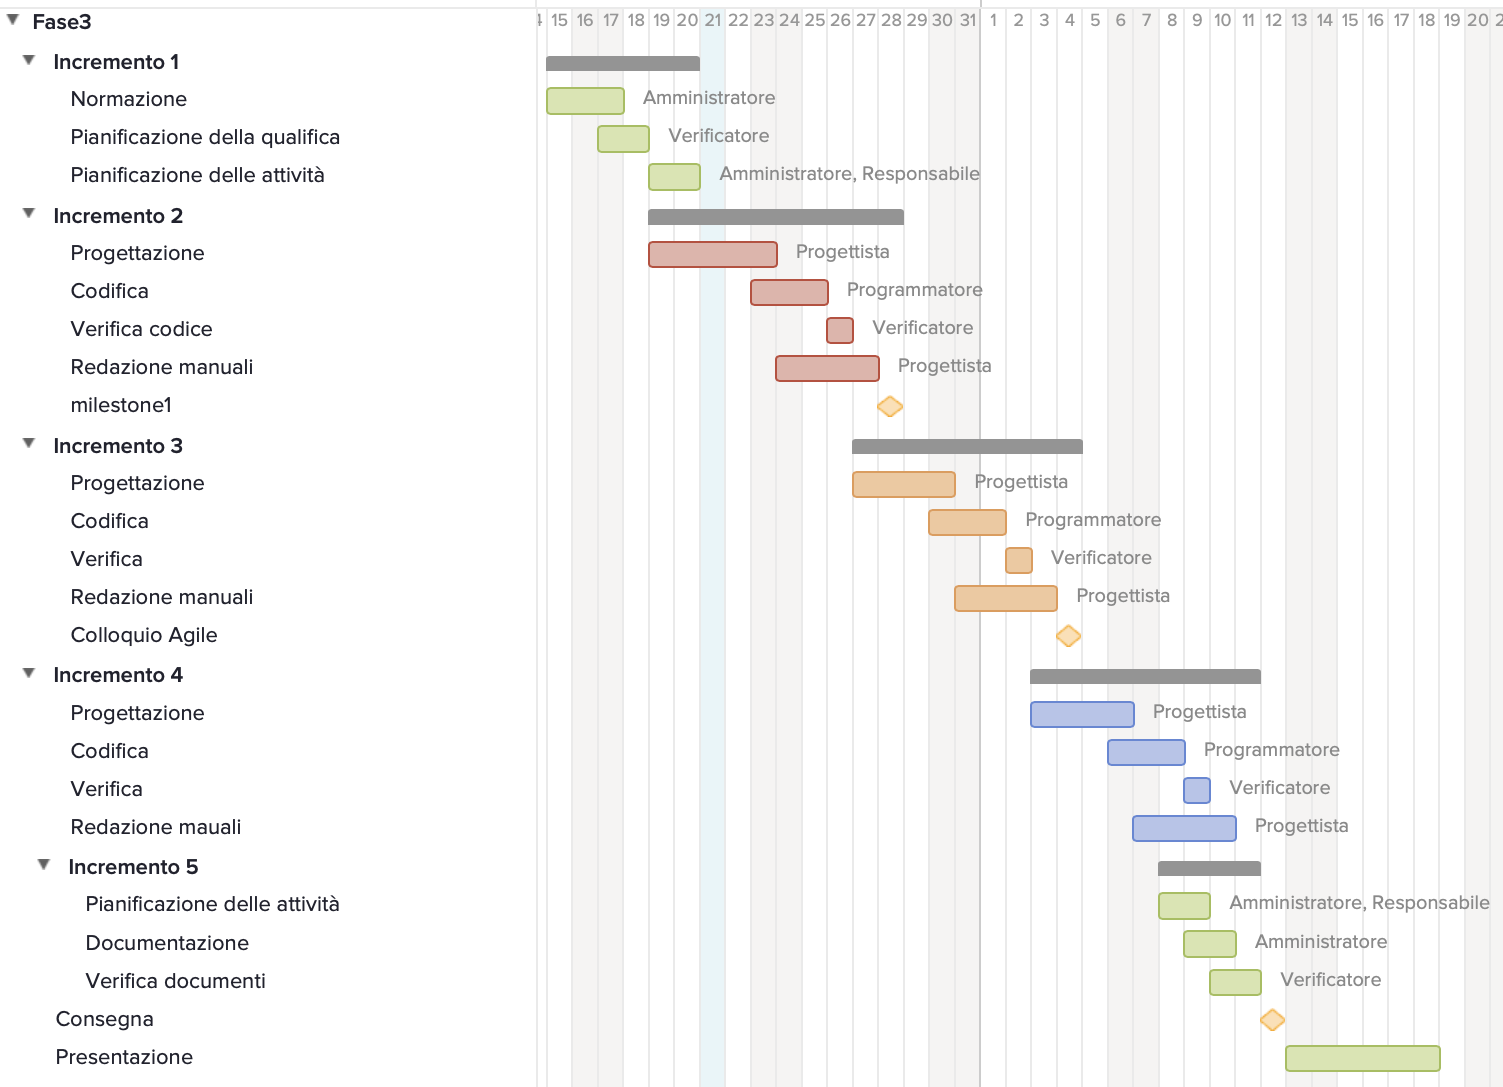
\includegraphics[scale=0.60]{images/fase3.png}
	\caption{Diagramma di Gantt riguardante la fase 3}
\end{figure}